% PP-Article.tex for AEA last revised 22 June 2011
%\documentclass[draftmode]{AEA}
\documentclass[AER]{AEA}

%\documentclass[12pt, a4paper]{article}
% If you have trouble with the mathtime package please see our technical support 
% document at: http://www.aeaweb.org/templates/technical_support.pdf
% You may remove the mathtime package if you can't get it working but your page
% count may be inaccurate as a result.
%\usepackage[cmbold]{mathtime}

% Note: you may use either harvard or natbib (but not both) to provide a wider
% variety of citation commands than latex supports natively. See below.

% Uncomment the next line to use the natbib package with bibtex 
\usepackage{natbib}

% Uncomment the next line to use the harvard package with bibtex
%\usepackage[abbr]{harvard}

%other packages
\usepackage{booktabs} % Allows the use of \toprule, \midrule and \bottomrule in tables
\usepackage{comment}
\usepackage{xcolor}
\usepackage{hyperref}
\usepackage{amsmath,amssymb,amsthm}
\usepackage{graphicx} % Allows including images
\usepackage{multicol}
\usepackage{multirow}
\usepackage{forest}
\usepackage{lscape}
\usepackage{adjustbox}
\usepackage{multicol}
\setlength{\columnsep}{1cm}
\usepackage{pgf,tikz}
\usepackage{subcaption} %for subfigure
%\usepackage{float} %For better positioning of objects
\forestset{qtree/.style={for tree={parent anchor=south, 
           child anchor=north,align=center,inner sep=0pt}}}

\usepackage{progressbar}

\usepackage{csquotes}
\usepackage{setspace}
           

%For number in equations with 'align'
\newcommand{\tabnotes}[2]{\bottomrule \multicolumn{#1}{@{}p{0.70\linewidth}@{}}{\footnotesize #2 }\end{tabular}\end{table}}

\newcommand\numberthis{\addtocounter{equation}{1}\tag{\theequation}} %https://tex.stackexchange.com/questions/42726/align-but-show-one-equation-number-at-the-end


%For quotting we define this 2:
\SetBlockThreshold{2}
\newcommand\myblockquote[2]{%
  \blockquote{\hspace*{2em}\emph{`#1'}\hfill(#2)}\par}


%For links
\definecolor{darkblue}{rgb}{0.0, 0.0, 0.65}
\definecolor{darkgreen}{rgb}{0.0, 0.65, 0.0}
\hypersetup{
	citecolor=blue,
	colorlinks=true,
	linkcolor=blue,
	filecolor=magenta,
	urlcolor=magenta
}

\let\footnote\thanks
%Prevent Footnote from breaking pages
\interfootnotelinepenalty=10000

%\usepackage[round]{natbib}


% This command determines the leading (vertical space between lines) in draft mode
% with 1.5 corresponding to "double" spacing.
\draftSpacing{1.5}

\begin{document}

%Has information on all the statistics estimated
\input{./macros.tex} 

%Full text

\title{When the Household Becomes the School: Sibling Effects on Parental Attention and Educational Outcomes During School Closures} %Sibling Spillovers from College Admission: Impacts on School Performance and Parental Expectations
\shortTitle{School closures and family size}
\author{
	Francisco Pardo \\
    \textit{\textcolor{red}{Preliminary Draft: Do Not Circulate}}
    %\textbf{University of Texas at Austin \footnote{\textit{Address:} 2908 Pearl Street APT C, Austin, Texas, 78705. \textit{phone:} +1 (202) 412-3049. \textit{email:} fpardo\@utexas.edu. \textit{webpage:} francisco-pardo-pajuelo.github.io.}}
	%\and
    %Author 2 \\
    %\textbf{Institution 2}
}
\date{\today}
%\pubMonth{}
%\pubYear{}
%\pubVolume{}
%\pubIssue{}
\JEL{}
\Keywords{}
%
\begin{abstract}


\\
\textit{JEL Codes: I21, I24}
\end{abstract}

%   I2 Education and Research Institutions
    % 	I20 	General 
    %   I21 	Analysis of Education
    %	I23 	Higher Education • Research Institutions
    %	I24 	Education and Inequality
    %	I26 	Returns to Education 
    %   I28 	Government Policy     
    
%   D1 	Household Behavior and Family Economics 
    % 	D13 	Household Production and Intrahousehold Allocation 
    %   D19  other

%   J2 	Demand and Supply of Labor 
    %   J24 	Human Capital • Skills • Occupational Choice • Labor Productivity 

%   O1 	Economic Development 
    %   O15 	Human Resources • Human Development • Income Distribution • Migration 

%   R2 	Household Analysis  
    % 	R23 	Regional Migration • Regional Labor Markets • Population • Neighborhood Characteristics 






\maketitle
The COVID-19 pandemic shifted educational responsibilities from schools to households. This allows me to examine the quantity-quality tradeoff in a context where parents play a larger role in childcare and education. Sibling spillovers might occur through direct effects (mentoring or competing for resources like computers) or indirect effects through parental resource allocation, as increased childcare reduces time for educational activities. With reduced participation from schools and teachers in students’ education and children being at home, parental investments in education become more important but more constrained due to increased childcare responsibilities; hence, these sibling spillovers may be exacerbated. 
%There are many different potential mechanisms through which these sibling spillovers might occur. On the one hand, siblings might have a direct effect on one another, positively through mentoring or negatively by competing for limited resources such as a computer. On the other hand, they might also have an indirect effect on one another through their effect on the allocation of parental resources, such as additional time required for childcare that could reduce time invested in educational activities.

I study the differential impact of learning losses between students with siblings and only children in this context. First, I use international PISA scores and UNESCO school closure data. In \hyperref[fig:pisa]{Figure \ref{fig:pisa}}, I show that across developed and developing countries, learning losses have been higher for students with siblings, and the size of these differential losses is correlated with the duration of school closures. Then I use administrative data from Peru from 2014 to 2024 on school progression and standardized exams using parents' IDs to identify siblings within the data. I find that relative to only children, children with siblings do much worse when the pandemic begins, with larger effects for larger families of up to 0.1 standard deviations (\hyperref[fig:event_study]{Figure \ref{fig:event_study}}). Moreover, they are robust and present regardless of parental education and other potential attenuating factors (\hyperref[fig:twfe]{Figure \ref{fig:twfe}}). Finally, to explore potential mechanisms behind this, I exploit school-starting age cutoffs as exogenous variation in parental investments. In normal circumstances, having a younger sibling delay their school start could imply more time required for childcare and less time available for investing in the children already in school, affecting their performance. In \hyperref[tab:rd_gpa]{Table \ref{tab:rd_gpa}} and \hyperref[tab:rd_ece]{Table \ref{tab:rd_ece}}, I find evidence that this is the case in years before and after the pandemic, where delaying school starting age increases childcare responsibilities, but not during the pandemic, when all children were already at home. This suggests that increased childcare responsibilities during school closures may create similar spillover effects on siblings.



 %I find that (i) across developed and developing countries, learning losses have been higher for students with siblings and the size of these differential losses is correlated with the duration of school closures , (ii) In Peru, I observe that this happens regardless of socioeconomic status, internet access, parental education and other potential attenuating factors and (iii) that these effects are partially caused by the increased responsibilities in childcare and education that parents need to take on the rest of their children and (iv) that the differential impact continues to be present even 4 years after the closures, highlighting potential changes in norms and beliefs about the way parental investment affects the education production function.

\newpage


\begin{figure}[htbp]
    \centering
    
        \centering
        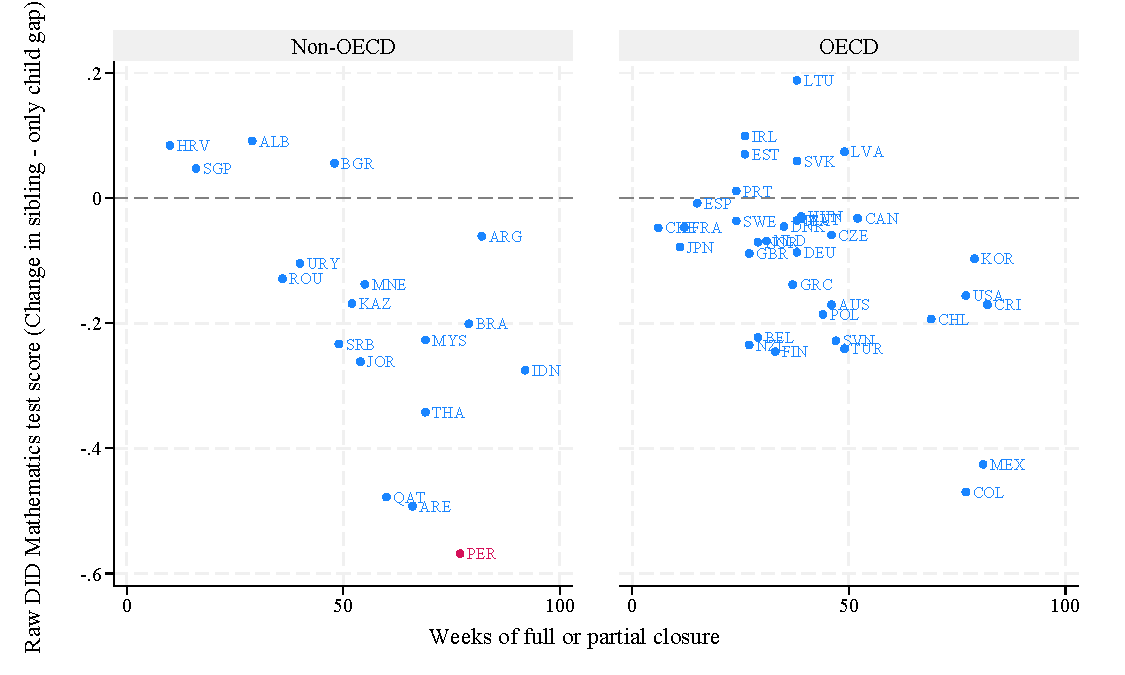
\includegraphics[width=0.9\textwidth]{./FIGURES/Descriptive/PISA_raw_DID_PV1MATH_not_fully_open.pdf}
        %\caption{Change in learning gaps by duration of school closure for OECD and Non-OECD countries.}
    
    \caption{Change in learning gaps by duration of school closure for OECD and Non-OECD countries.}
    \label{fig:pisa}
\end{figure}

\begin{figure}[htbp]
    \centering
    
        \centering
        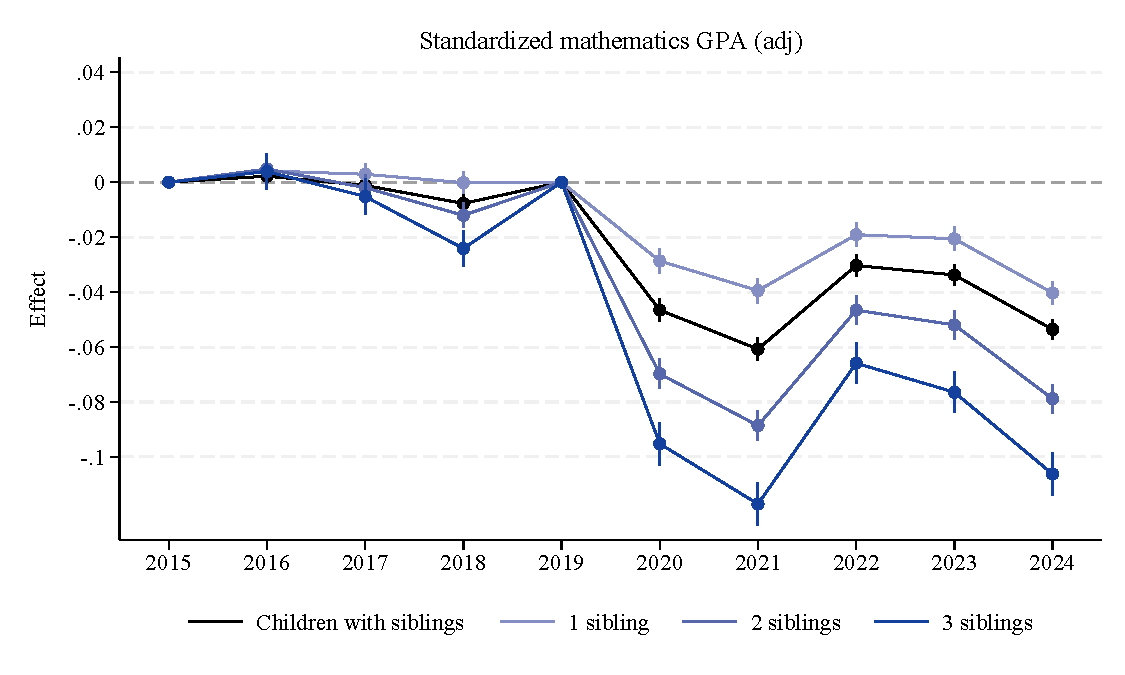
\includegraphics[width=0.9\textwidth]{./FIGURES/Event Study/covid_std_gpa_m_adj_all_all_all_elm_all.pdf}
        %\caption{Change in learning gaps by duration of school closure for OECD and Non-OECD countries.}
    
    \caption{Event Study: Learning losses of children with siblings overall and by number of siblings compared to only children}
    \label{fig:event_study}
\end{figure}


\begin{figure}[htbp]
    \centering
    
        \centering
        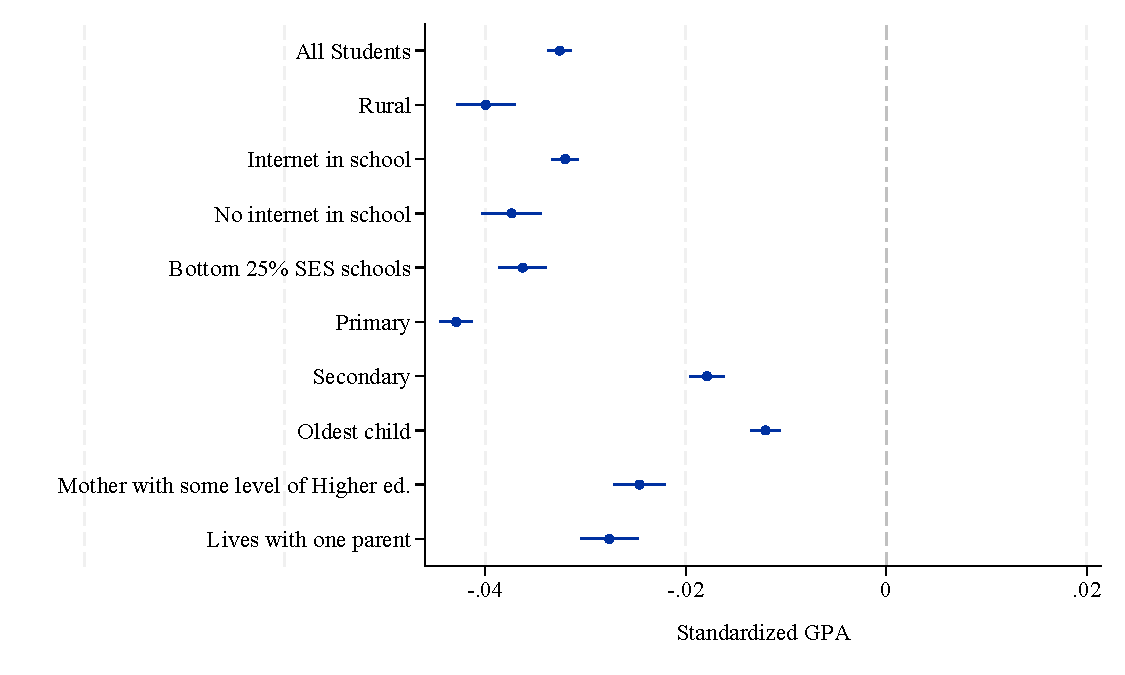
\includegraphics[width=\textwidth]{./FIGURES/TWFE/covid_twfe_summ_all_all_gpa_m_adj_4.pdf}
        %\caption{Change in learning gaps by duration of school closure for OECD and Non-OECD countries.}
        
    
    \caption{Difference in Difference: Learning losses of children with siblings compared to only children by different subsamples.}\label{fig:twfe}
\end{figure}



%RD-first grade
\begin{table}[htbp]
\centering
\caption{Effect of Younger Sibling Delayed School Entry on Standardized GPA before, during and after the Pandemic}
\label{tab:rd_gpa}
\resizebox{0.9\textwidth}{!}{
\begin{tabular}{lccc}
\toprule
\cmidrule(lr){2-4}
& \multicolumn{3}{c}{Standardized GPA} \\
\cmidrule(lr){2-4}
& Pre-Covid & Covid & Post-Covid  \\
& 2018-2019 & 2020-2021 & 2022-2023  \\
\cmidrule(lr){2-2} \cmidrule(lr){3-3} \cmidrule(lr){4-4}
& (1) & (2) & (3)  \\
\bottomrule
&  &  &   \\
Delay School (After SSA)&      -0.023***&      -0.001   &      -0.023***\\
                    &     (0.007)   &     (0.007)   &     (0.006)   \\
Local Linear        &         Yes   &         Yes   &         Yes   \\
                    &               &               &               \\
Observations        &     358,861   &     354,044   &     447,536   \\
Counterfactual mean &       0.058   &       0.020   &       0.050   \\
Bandwidth           &         365   &         365   &         365   \\
 

\bottomrule
\end{tabular}
}
\begin{tablenotes}
\footnotesize
This table presents local linear regression discontinuity estimates of the effect of having a younger sibling delay school entry (after reaching school starting age, SSA) on the older sibling standardized GPA across three time periods: pre-Covid (2018-2019), Covid (2020-2021), and post-Covid (2022-2023). All specifications use a bandwidth of 365 days around the school entry cutoff. Robust standard errors are reported in parentheses. The counterfactual mean represents the predicted GPA for students just below the cutoff (those who entered school on time). *** p<0.01, ** p<0.05, * p<0.1.
\end{tablenotes}
\end{table}


\newpage
\begin{table}[htbp]
\centering
\caption{Effect of Younger Sibling Delayed School Entry on Standardized Exams and Parental Investment}
\label{tab:rd_ece}
\resizebox{\textwidth}{!}{
\begin{tabular}{lccccc}
\toprule
& \multicolumn{2}{c}{Pre-Covid}  & \multicolumn{3}{c}{Post-Covid} \\
& \multicolumn{2}{c}{2018-2019}  & \multicolumn{3}{c}{2022-2024}  \\
\cmidrule(lr){2-3} \cmidrule(lr){4-6}
& Mathematics & Reading & Mathematics & Reading & Parental Investment  \\
& (1) & (2) & (3) & (4) & (5) \\
\bottomrule
&  &  &  & &  \\
\multirow{2}{*}{\shortstack[l]{Younger sibling born after \\ school-entry cutoff}}&      -0.023*  &      -0.023*  &      -0.011   &      -0.012   &      -0.038***\\
                    &     (0.014)   &     (0.012)   &     (0.013)   &     (0.010)   &     (0.013)   \\
Local Linear        &         Yes   &         Yes   &         Yes   &         Yes   &         Yes   \\
                    &               &               &               &               &               \\
Observations        &      87,927   &      87,924   &     106,174   &     106,257   &     102,901   \\
Counterfactual mean &      -0.110   &      -0.087   &       0.189   &       0.284   &      -0.005   \\
Bandwidth           &         365   &         365   &         365   &         365   &         365   \\
 

\bottomrule
\end{tabular}
}
\begin{tablenotes}
\footnotesize
 This table presents local linear regression discontinuity estimates of the effect of having a younger sibling delay school entry (after reaching school starting age, SSA) on the older sibling standardized national examinations and parental investment in education across two time periods: pre-Covid (2018-2019) and post-Covid (2022-2023). The parental investment index has been calculated based on several questions related to time spent with the children in educational activities. All specifications use a bandwidth of 365 days around the school entry cutoff. Robust standard errors are reported in parentheses. The counterfactual mean represents the predicted GPA for students just below the cutoff (those who entered school on time). *** p<0.01, ** p<0.05, * p<0.1.
\end{tablenotes}
\end{table}




%\clearpage
%\newpage

\setcounter{figure}{0}
\renewcommand\thefigure{A.\arabic{figure}}    

\setcounter{table}{0}
\renewcommand{\thetable}{A.\arabic{table}}


\begin{center}
\huge
\textbf{Appendix: NOT FOR PUBLICATION}
\normalsize
\end{center}


\section*{Appendix A: Robustness} \label{sec:appa}
\newpage


\makebox[0.1\width][l]{
\resizebox{\textwidth}{!}{
\begin{tabular}{lccc}
\toprule
\cmidrule(lr){2-4}
& \multicolumn{3}{c}{Standardized GPA}
\cmidrule(lr){2-4}
& Pre-Covid & Covid & Post-Covid  \\
& 2018-2019 & 2020-2021 & 2022-2023  \\
\cmidrule(lr){2-2} \cmidrule(lr){3-3} \cmidrule(lr){4-4}
& (1) & (2) & (3)  \\
\bottomrule
&  &  &   \\
Delay School (After SSA)&      -0.001   &      -0.010   &      -0.004   \\
                    &     (0.006)   &     (0.006)   &     (0.006)   \\
Local Linear        &         Yes   &         Yes   &         Yes   \\
                    &               &               &               \\
Observations        &     418,987   &     371,966   &     485,601   \\
Counterfactual mean &       0.043   &       0.020   &       0.031   \\
Bandwidth           &         365   &         365   &         365   \\
 

\bottomrule
\end{tabular}
}
}


\newpage

\makeatletter
\@ifclassloaded{beamer}{%
       \centering
       \resizebox{0.6\textwidth}{!}%
}{%
       \begin{table}[!tbp]\centering\def\sym#1{\ifmmode^{#1}\else\(^{#1}\)\fi}
       \centering
       \caption{Effects of younger sibling delaying school on older sibling standardized exams - 2 - m - a -  - 365}
       \label{tab:rd_summ_2_m_a_365}
       \resizebox{0.95\textwidth}{!}%
}
{
\makeatother
\makebox[0.1\width][l]{
\resizebox{\textwidth}{!}{
\begin{tabular}{lccc}
\toprule
\cmidrule(lr){2-4}
& \multicolumn{3}{c}{Standardized GPA} \\
\cmidrule(lr){2-4}
& Pre-Covid & Covid & Post-Covid  \\
& 2018-2019 & 2020-2021 & 2022-2023  \\
\cmidrule(lr){2-2} \cmidrule(lr){3-3} \cmidrule(lr){4-4}
& (1) & (2) & (3)  \\
\bottomrule
&  &  &   \\
\multirow{2}{*}{\shortstack[l]{Younger sibling born after \\ school-entry cutoff}}&      -0.000   &      -0.008   &       0.001   \\
                    &     (0.008)   &     (0.007)   &     (0.007)   \\
Local Linear        &         Yes   &         Yes   &         Yes   \\
                    &               &               &               \\
Observations        &     268,561   &     288,245   &     357,788   \\
Counterfactual mean &       0.053   &       0.027   &       0.053   \\
Bandwidth           &         365   &         365   &         365   \\
 

\bottomrule
\end{tabular}
}
\@ifclassloaded{beamer}{%
}{%
       \end{table}
}


\makeatletter
\@ifclassloaded{beamer}{%
       \centering
       \resizebox{0.6\textwidth}{!}%
}{%
       \begin{table}[!tbp]\centering\def\sym#1{\ifmmode^{#1}\else\(^{#1}\)\fi}
       \centering
       \caption{TWFE on GPA by baseline resources}
       \label{tab:twfe_ece_survey_1_pair1}
       \resizebox{0.65\textwidth}{!}%
}
{
\makeatother
\begin{tabular}{lccc}
\toprule
\cmidrule(lr){2-4}
& \multicolumn{3}{c}{TWFE} \\
\cmidrule(lr){2-4}
& 1 sibling & 2 siblings & 3 siblings  \\
\cmidrule(lr){2-2} \cmidrule(lr){3-3} \cmidrule(lr){4-4}
& (1) & (2) & (3)\\
\bottomrule
&  &  &  \\
&  &  &   \\
\multicolumn{4}{l}{\textit{Panel A: All studentes}} \\
\hspace{3mm}Mathematics&      -0.046***&      -0.078***&      -0.077** \\
                    &     (0.013)   &     (0.018)   &     (0.035)   \\
 
%&  &  &   \\
\hspace{3mm}Reading &      -0.023*  &      -0.035*  &      -0.072** \\
                    &     (0.013)   &     (0.018)   &     (0.035)   \\
                    &               &               &               \\
\hspace{3mm}Observations&     108,585   &      85,464   &      72,938   \\
 
&  &  &   \\
\multicolumn{4}{l}{\textit{Panel B: Low SES Households (Q1)}} \\
\hspace{3mm}Mathematics&      -0.026   &      -0.029   &      -0.166***\\
                    &     (0.026)   &     (0.033)   &     (0.057)   \\
 
%&  &  &   \\
\hspace{3mm}Reading &       0.001   &      -0.001   &      -0.133** \\
                    &     (0.026)   &     (0.034)   &     (0.058)   \\
                    &               &               &               \\
\hspace{3mm}Observations&      25,600   &      20,717   &      17,069   \\
 
&  &  &   \\
\multicolumn{4}{l}{\textit{Panel C: High SES Households (Q4)}} \\
\hspace{3mm}Mathematics&      -0.069** &       0.013   &       0.034   \\
                    &     (0.034)   &     (0.056)   &     (0.155)   \\
 
%&  &  &   \\
\hspace{3mm}Reading &      -0.026   &      -0.045   &       0.279*  \\
                    &     (0.034)   &     (0.056)   &     (0.153)   \\
                    &               &               &               \\
\hspace{3mm}Observations&      18,418   &      13,891   &      12,219   \\
 
&  &  &   \\
\multicolumn{4}{l}{\textit{Panel D: Households with no PC or Internet}} \\
\hspace{3mm}Mathematics&      -0.057***&      -0.113***&      -0.058   \\
                    &     (0.020)   &     (0.027)   &     (0.051)   \\
 
%&  &  &   \\
\hspace{3mm}Reading &      -0.036*  &      -0.033   &      -0.069   \\
                    &     (0.020)   &     (0.027)   &     (0.051)   \\
                    &               &               &               \\
\hspace{3mm}Observations&      46,281   &      36,305   &      30,041   \\
 
&  &  &   \\
\multicolumn{4}{l}{\textit{Panel E: Households with both PC and Internet}} \\
\hspace{3mm}Mathematics&      -0.013   &       0.015   &       0.307** \\
                    &     (0.034)   &     (0.056)   &     (0.146)   \\
 
%&  &  &   \\
\hspace{3mm}Reading &       0.009   &       0.006   &       0.505***\\
                    &     (0.035)   &     (0.056)   &     (0.147)   \\
                    &               &               &               \\
\hspace{3mm}Observations&      18,086   &      13,736   &      12,097   \\
 

\bottomrule
\end{tabular}
}
\@ifclassloaded{beamer}{%
}{%
       \end{table}
}

\makeatletter
\@ifclassloaded{beamer}{%
       \centering
       \resizebox{0.6\textwidth}{!}%
}{%
       \begin{table}[!tbp]\centering\def\sym#1{\ifmmode^{#1}\else\(^{#1}\)\fi}
       \centering
       \caption{TWFE on GPA by baseline resources}
       \label{tab:twfe_ece_survey_1_pair2}
       \resizebox{0.65\textwidth}{!}%
}
{
\makeatother
\begin{tabular}{lccc}
\toprule
\cmidrule(lr){2-4}
& \multicolumn{3}{c}{TWFE} \\
\cmidrule(lr){2-4}
& 1 sibling & 2 siblings & 3 siblings  \\
\cmidrule(lr){2-2} \cmidrule(lr){3-3} \cmidrule(lr){4-4}
& (1) & (2) & (3)\\
\bottomrule
&  &  &  \\
&  &  &   \\
\multicolumn{4}{l}{\textit{Panel A: All studentes}} \\
\hspace{3mm}Mathematics&      -0.024***&      -0.062***&      -0.110***\\
                    &     (0.007)   &     (0.010)   &     (0.019)   \\
 
%&  &  &   \\
\hspace{3mm}Reading &      -0.014** &      -0.064***&      -0.077***\\
                    &     (0.007)   &     (0.010)   &     (0.020)   \\
                    &               &               &               \\
\hspace{3mm}Observations&     341,265   &     272,263   &     236,637   \\
 
&  &  &   \\
\multicolumn{4}{l}{\textit{Panel B: Low SES Households (Q1)}} \\
\hspace{3mm}Mathematics&      -0.014   &      -0.048** &      -0.131***\\
                    &     (0.015)   &     (0.019)   &     (0.031)   \\
 
%&  &  &   \\
\hspace{3mm}Reading &      -0.004   &      -0.050***&      -0.073** \\
                    &     (0.015)   &     (0.019)   &     (0.031)   \\
                    &               &               &               \\
\hspace{3mm}Observations&      73,524   &      61,008   &      51,297   \\
 
&  &  &   \\
\multicolumn{4}{l}{\textit{Panel C: High SES Households (Q4)}} \\
\hspace{3mm}Mathematics&      -0.038** &      -0.041   &      -0.203***\\
                    &     (0.016)   &     (0.028)   &     (0.073)   \\
 
%&  &  &   \\
\hspace{3mm}Reading &      -0.029*  &      -0.047*  &      -0.043   \\
                    &     (0.016)   &     (0.028)   &     (0.074)   \\
                    &               &               &               \\
\hspace{3mm}Observations&      70,576   &      54,091   &      48,686   \\
 
&  &  &   \\
\multicolumn{4}{l}{\textit{Panel D: Households with no PC or Internet}} \\
\hspace{3mm}Mathematics&      -0.027*  &      -0.054** &      -0.084*  \\
                    &     (0.014)   &     (0.021)   &     (0.048)   \\
 
%&  &  &   \\
\hspace{3mm}Reading &      -0.015   &      -0.054***&      -0.057   \\
                    &     (0.014)   &     (0.021)   &     (0.048)   \\
                    &               &               &               \\
\hspace{3mm}Observations&     104,804   &      84,220   &      73,029   \\
 
&  &  &   \\
\multicolumn{4}{l}{\textit{Panel E: Households with both PC and Internet}} \\
\hspace{3mm}Mathematics&      -0.036***&      -0.032*  &      -0.144***\\
                    &     (0.012)   &     (0.019)   &     (0.041)   \\
 
%&  &  &   \\
\hspace{3mm}Reading &      -0.027** &      -0.051***&      -0.064   \\
                    &     (0.013)   &     (0.019)   &     (0.042)   \\
                    &               &               &               \\
\hspace{3mm}Observations&     125,843   &      98,884   &      85,077   \\
 

\bottomrule
\end{tabular}
}
\@ifclassloaded{beamer}{%
}{%
       \end{table}
}

\makeatletter
\@ifclassloaded{beamer}{%
       \centering
       \resizebox{0.6\textwidth}{!}%
}{%
       \begin{table}[!tbp]\centering\def\sym#1{\ifmmode^{#1}\else\(^{#1}\)\fi}
       \centering
       \caption{TWFE on 7th grade GPA by 4th grade baseline resources}
       \label{tab:twfe_gpa_baseline_survey_1_pair3}
       \resizebox{0.65\textwidth}{!}%
}
{
\makeatother
\begin{tabular}{lccc}
\toprule
\cmidrule(lr){2-4}
& \multicolumn{3}{c}{TWFE} \\
\cmidrule(lr){2-4}
& 1 sibling & 2 siblings & 3 siblings  \\
\cmidrule(lr){2-2} \cmidrule(lr){3-3} \cmidrule(lr){4-4}
& (1) & (2) & (3)\\
\bottomrule
&  &  &  \\
&  &  &   \\
\multicolumn{4}{l}{\textit{Panel A: All studentes}} \\
\hspace{3mm}Mathematics&      -0.024***&      -0.070***&      -0.060***\\
                    &     (0.007)   &     (0.010)   &     (0.018)   \\
 
%&  &  &   \\
\hspace{3mm}Reading &      -0.021***&      -0.045***&      -0.033*  \\
                    &     (0.007)   &     (0.010)   &     (0.018)   \\
                    &               &               &               \\
\hspace{3mm}Observations&     365,702   &     292,698   &     254,104   \\
 
&  &  &   \\
\multicolumn{4}{l}{\textit{Panel B: Low SES Households (Q1)}} \\
\hspace{3mm}Mathematics&      -0.000   &      -0.020   &      -0.005   \\
                    &     (0.014)   &     (0.017)   &     (0.028)   \\
 
%&  &  &   \\
\hspace{3mm}Reading &      -0.012   &      -0.006   &       0.004   \\
                    &     (0.014)   &     (0.017)   &     (0.028)   \\
                    &               &               &               \\
\hspace{3mm}Observations&      90,252   &      75,485   &      63,910   \\
 
&  &  &   \\
\multicolumn{4}{l}{\textit{Panel C: High SES Households (Q4)}} \\
\hspace{3mm}Mathematics&      -0.026*  &      -0.091***&      -0.106   \\
                    &     (0.016)   &     (0.027)   &     (0.071)   \\
 
%&  &  &   \\
\hspace{3mm}Reading &      -0.031** &      -0.097***&      -0.066   \\
                    &     (0.016)   &     (0.027)   &     (0.072)   \\
                    &               &               &               \\
\hspace{3mm}Observations&      73,259   &      56,234   &      50,652   \\
 
&  &  &   \\
\multicolumn{4}{l}{\textit{Panel D: Households with no PC or Internet}} \\
\hspace{3mm}Mathematics&      -0.018   &      -0.107***&      -0.084*  \\
                    &     (0.013)   &     (0.020)   &     (0.046)   \\
 
%&  &  &   \\
\hspace{3mm}Reading &      -0.021   &      -0.077***&      -0.107** \\
                    &     (0.013)   &     (0.020)   &     (0.047)   \\
                    &               &               &               \\
\hspace{3mm}Observations&     113,464   &      91,731   &      79,607   \\
 
&  &  &   \\
\multicolumn{4}{l}{\textit{Panel E: Households with both PC and Internet}} \\
\hspace{3mm}Mathematics&      -0.007   &      -0.023   &      -0.003   \\
                    &     (0.012)   &     (0.018)   &     (0.040)   \\
 
%&  &  &   \\
\hspace{3mm}Reading &       0.006   &      -0.030*  &      -0.016   \\
                    &     (0.012)   &     (0.018)   &     (0.040)   \\
                    &               &               &               \\
\hspace{3mm}Observations&     136,957   &     108,035   &      92,888   \\
 

\bottomrule
\end{tabular}
}
\@ifclassloaded{beamer}{%
}{%
       \end{table}
}

\makeatletter
\@ifclassloaded{beamer}{%
       \centering
       \resizebox{0.6\textwidth}{!}%
}{%
       \begin{table}[!tbp]\centering\def\sym#1{\ifmmode^{#1}\else\(^{#1}\)\fi}
       \centering
       \caption{TWFE on GPA by baseline resources}
       \label{tab:twfe_ece_survey_1_pair4}
       \resizebox{0.65\textwidth}{!}%
}
{
\makeatother
\begin{tabular}{lccc}
\toprule
\cmidrule(lr){2-4}
& \multicolumn{3}{c}{TWFE} \\
\cmidrule(lr){2-4}
& 1 sibling & 2 siblings & 3 siblings  \\
\cmidrule(lr){2-2} \cmidrule(lr){3-3} \cmidrule(lr){4-4}
& (1) & (2) & (3)\\
\bottomrule
&  &  &  \\
&  &  &   \\
\multicolumn{4}{l}{\textit{Panel A: All studentes}} \\
\hspace{3mm}Mathematics&      -0.032***&      -0.053***&      -0.074***\\
                    &     (0.006)   &     (0.008)   &     (0.014)   \\
 
%&  &  &   \\
\hspace{3mm}Reading &      -0.018***&      -0.035***&      -0.045***\\
                    &     (0.006)   &     (0.008)   &     (0.014)   \\
                    &               &               &               \\
\hspace{3mm}Observations&     466,128   &     384,809   &     339,142   \\
 
&  &  &   \\
\multicolumn{4}{l}{\textit{Panel B: Low SES Households (Q1)}} \\
\hspace{3mm}Mathematics&      -0.018   &      -0.023   &      -0.044** \\
                    &     (0.012)   &     (0.015)   &     (0.021)   \\
 
%&  &  &   \\
\hspace{3mm}Reading &      -0.002   &      -0.006   &      -0.045** \\
                    &     (0.012)   &     (0.015)   &     (0.022)   \\
                    &               &               &               \\
\hspace{3mm}Observations&     119,170   &     103,085   &      90,231   \\
 
&  &  &   \\
\multicolumn{4}{l}{\textit{Panel C: High SES Households (Q4)}} \\
\hspace{3mm}Mathematics&      -0.039***&      -0.074***&      -0.091*  \\
                    &     (0.013)   &     (0.021)   &     (0.050)   \\
 
%&  &  &   \\
\hspace{3mm}Reading &      -0.026*  &      -0.057***&      -0.027   \\
                    &     (0.013)   &     (0.022)   &     (0.050)   \\
                    &               &               &               \\
\hspace{3mm}Observations&      91,916   &      72,508   &      64,890   \\
 
&  &  &   \\
\multicolumn{4}{l}{\textit{Panel D: Households with no PC or Internet}} \\
\hspace{3mm}Mathematics&      -0.032***&      -0.059***&      -0.063** \\
                    &     (0.009)   &     (0.014)   &     (0.029)   \\
 
%&  &  &   \\
\hspace{3mm}Reading &      -0.021** &      -0.036** &       0.004   \\
                    &     (0.010)   &     (0.014)   &     (0.030)   \\
                    &               &               &               \\
\hspace{3mm}Observations&     186,154   &     149,785   &     133,378   \\
 
&  &  &   \\
\multicolumn{4}{l}{\textit{Panel E: Households with both PC and Internet}} \\
\hspace{3mm}Mathematics&      -0.031***&      -0.042***&      -0.095***\\
                    &     (0.010)   &     (0.013)   &     (0.020)   \\
 
%&  &  &   \\
\hspace{3mm}Reading &      -0.005   &      -0.030** &      -0.066***\\
                    &     (0.011)   &     (0.013)   &     (0.021)   \\
                    &               &               &               \\
\hspace{3mm}Observations&     153,436   &     130,307   &     113,257   \\
 

\bottomrule
\end{tabular}
}
\@ifclassloaded{beamer}{%
}{%
       \end{table}
}


\makeatletter
\@ifclassloaded{beamer}{%
       \centering
       \resizebox{0.6\textwidth}{!}%
}{%
       \begin{table}[!tbp]\centering\def\sym#1{\ifmmode^{#1}\else\(^{#1}\)\fi}
       \centering
       \caption{TWFE on 6th grade GPA by 2nd grade baseline achievement and expectations}
       \label{tab:twfe_gpa_baseline_survey_2_pair1}
       \resizebox{0.65\textwidth}{!}%
}
{
\makeatother
\begin{tabular}{lccc}
\toprule
\cmidrule(lr){2-4}
& \multicolumn{3}{c}{TWFE} \\
\cmidrule(lr){2-4}
& 1 sibling & 2 siblings & 3 siblings  \\
\cmidrule(lr){2-2} \cmidrule(lr){3-3} \cmidrule(lr){4-4}
& (1) & (2) & (3)\\
\bottomrule
&  &  &  \\
&  &  &   \\
\multicolumn{4}{l}{\textit{Panel A: All studentes}} \\
\hspace{3mm}Mathematics&      -0.046***&      -0.078***&      -0.077** \\
                    &     (0.013)   &     (0.018)   &     (0.035)   \\
 
%&  &  &   \\
\hspace{3mm}Reading &      -0.023*  &      -0.035*  &      -0.072** \\
                    &     (0.013)   &     (0.018)   &     (0.035)   \\
                    &               &               &               \\
\hspace{3mm}Observations&     108,585   &      85,464   &      72,938   \\
 
&  &  &   \\
\multicolumn{4}{l}{\textit{Panel B: Student in bottom quartile of achievement}} \\
\hspace{3mm}Mathematics&      -0.028   &      -0.073*  &      -0.160** \\
                    &     (0.032)   &     (0.041)   &     (0.072)   \\
 
%&  &  &   \\
\hspace{3mm}Reading &       0.018   &      -0.026   &      -0.095   \\
                    &     (0.032)   &     (0.042)   &     (0.073)   \\
                    &               &               &               \\
\hspace{3mm}Observations&      14,632   &      11,987   &      10,145   \\
 
&  &  &   \\
\multicolumn{4}{l}{\textit{Panel C: Student in top quartile of achievement}} \\
\hspace{3mm}Mathematics&      -0.061** &      -0.103***&       0.030   \\
                    &     (0.026)   &     (0.038)   &     (0.083)   \\
 
%&  &  &   \\
\hspace{3mm}Reading &      -0.049*  &      -0.044   &       0.009   \\
                    &     (0.026)   &     (0.038)   &     (0.084)   \\
                    &               &               &               \\
\hspace{3mm}Observations&      34,500   &      26,134   &      22,113   \\
 
&  &  &   \\
\multicolumn{4}{l}{\textit{Panel D: Max Expectation: Finish school}} \\
\hspace{3mm}Mathematics&       0.004   &      -0.078   &      -0.222   \\
                    &     (0.063)   &     (0.083)   &     (0.141)   \\
 
%&  &  &   \\
\hspace{3mm}Reading &       0.037   &       0.004   &      -0.250*  \\
                    &     (0.064)   &     (0.085)   &     (0.145)   \\
                    &               &               &               \\
\hspace{3mm}Observations&       5,127   &       4,075   &       3,422   \\
 
&  &  &   \\
\multicolumn{4}{l}{\textit{Panel E: Max Expectation: 4-year college or grad school}} \\
\hspace{3mm}Mathematics&      -0.048***&      -0.073***&      -0.041   \\
                    &     (0.015)   &     (0.021)   &     (0.042)   \\
 
%&  &  &   \\
\hspace{3mm}Reading &      -0.030** &      -0.031   &      -0.041   \\
                    &     (0.015)   &     (0.021)   &     (0.043)   \\
                    &               &               &               \\
\hspace{3mm}Observations&      87,535   &      67,871   &      57,831   \\
 

\bottomrule
\end{tabular}
}
\@ifclassloaded{beamer}{%
}{%
       \end{table}
}

\makeatletter
\@ifclassloaded{beamer}{%
       \centering
       \resizebox{0.6\textwidth}{!}%
}{%
       \begin{table}[!tbp]\centering\def\sym#1{\ifmmode^{#1}\else\(^{#1}\)\fi}
       \centering
       \caption{TWFE on 6th grade GPA by 4th grade baseline achievement and expectations}
       \label{tab:twfe_gpa_baseline_survey_2_pair2}
       \resizebox{0.65\textwidth}{!}%
}
{
\makeatother
\begin{tabular}{lccc}
\toprule
\cmidrule(lr){2-4}
& \multicolumn{3}{c}{TWFE} \\
\cmidrule(lr){2-4}
& 1 sibling & 2 siblings & 3 siblings  \\
\cmidrule(lr){2-2} \cmidrule(lr){3-3} \cmidrule(lr){4-4}
& (1) & (2) & (3)\\
\bottomrule
&  &  &  \\
&  &  &   \\
\multicolumn{4}{l}{\textit{Panel A: All studentes}} \\
\hspace{3mm}Mathematics&      -0.024***&      -0.062***&      -0.110***\\
                    &     (0.007)   &     (0.010)   &     (0.019)   \\
 
%&  &  &   \\
\hspace{3mm}Reading &      -0.014** &      -0.064***&      -0.077***\\
                    &     (0.007)   &     (0.010)   &     (0.020)   \\
                    &               &               &               \\
\hspace{3mm}Observations&     341,265   &     272,263   &     236,637   \\
 
&  &  &   \\
\multicolumn{4}{l}{\textit{Panel B: Student in bottom quartile of achievement}} \\
\hspace{3mm}Mathematics&      -0.013   &      -0.052***&      -0.084** \\
                    &     (0.015)   &     (0.020)   &     (0.035)   \\
 
%&  &  &   \\
\hspace{3mm}Reading &      -0.005   &      -0.049** &      -0.078** \\
                    &     (0.015)   &     (0.020)   &     (0.035)   \\
                    &               &               &               \\
\hspace{3mm}Observations&      64,124   &      52,974   &      45,942   \\
 
&  &  &   \\
\multicolumn{4}{l}{\textit{Panel C: Student in top quartile of achievement}} \\
\hspace{3mm}Mathematics&      -0.038** &      -0.094***&      -0.098** \\
                    &     (0.015)   &     (0.022)   &     (0.048)   \\
 
%&  &  &   \\
\hspace{3mm}Reading &      -0.022   &      -0.071***&      -0.095*  \\
                    &     (0.015)   &     (0.023)   &     (0.049)   \\
                    &               &               &               \\
\hspace{3mm}Observations&      97,944   &      74,571   &      64,319   \\
 
&  &  &   \\
\multicolumn{4}{l}{\textit{Panel D: Max Expectation: Finish school}} \\
\hspace{3mm}Mathematics&      -0.021   &      -0.064*  &       0.062   \\
                    &     (0.030)   &     (0.039)   &     (0.065)   \\
 
%&  &  &   \\
\hspace{3mm}Reading &      -0.004   &      -0.082** &      -0.018   \\
                    &     (0.030)   &     (0.039)   &     (0.065)   \\
                    &               &               &               \\
\hspace{3mm}Observations&      22,087   &      18,509   &      15,822   \\
 
&  &  &   \\
\multicolumn{4}{l}{\textit{Panel E: Max Expectation: 4-year college or grad school}} \\
\hspace{3mm}Mathematics&      -0.028***&      -0.061***&      -0.136***\\
                    &     (0.008)   &     (0.012)   &     (0.024)   \\
 
%&  &  &   \\
\hspace{3mm}Reading &      -0.018** &      -0.062***&      -0.106***\\
                    &     (0.008)   &     (0.012)   &     (0.024)   \\
                    &               &               &               \\
\hspace{3mm}Observations&     270,591   &     212,753   &     184,893   \\
 

\bottomrule
\end{tabular}
}
\@ifclassloaded{beamer}{%
}{%
       \end{table}
}

\makeatletter
\@ifclassloaded{beamer}{%
       \centering
       \resizebox{0.6\textwidth}{!}%
}{%
       \begin{table}[!tbp]\centering\def\sym#1{\ifmmode^{#1}\else\(^{#1}\)\fi}
       \centering
       \caption{WFE on GPA by baseline achievement and expectations}
       \label{tab:twfe_gpa_baseline_survey_2_pair3}
       \resizebox{0.65\textwidth}{!}%
}
{
\makeatother
\begin{tabular}{lccc}
\toprule
\cmidrule(lr){2-4}
& \multicolumn{3}{c}{TWFE} \\
\cmidrule(lr){2-4}
& 1 sibling & 2 siblings & 3 siblings  \\
\cmidrule(lr){2-2} \cmidrule(lr){3-3} \cmidrule(lr){4-4}
& (1) & (2) & (3)\\
\bottomrule
&  &  &  \\
&  &  &   \\
\multicolumn{4}{l}{\textit{Panel A: All studentes}} \\
\hspace{3mm}Mathematics&      -0.024***&      -0.070***&      -0.060***\\
                    &     (0.007)   &     (0.010)   &     (0.018)   \\
 
%&  &  &   \\
\hspace{3mm}Reading &      -0.021***&      -0.045***&      -0.033*  \\
                    &     (0.007)   &     (0.010)   &     (0.018)   \\
                    &               &               &               \\
\hspace{3mm}Observations&     365,702   &     292,698   &     254,104   \\
 
&  &  &   \\
\multicolumn{4}{l}{\textit{Panel B: Student in bottom quartile of achievement}} \\
\hspace{3mm}Mathematics&       0.022   &      -0.009   &      -0.101***\\
                    &     (0.015)   &     (0.019)   &     (0.033)   \\
 
%&  &  &   \\
\hspace{3mm}Reading &       0.020   &      -0.005   &      -0.015   \\
                    &     (0.015)   &     (0.020)   &     (0.034)   \\
                    &               &               &               \\
\hspace{3mm}Observations&      76,396   &      63,590   &      55,311   \\
 
&  &  &   \\
\multicolumn{4}{l}{\textit{Panel C: Student in top quartile of achievement}} \\
\hspace{3mm}Mathematics&      -0.046***&      -0.118***&      -0.166***\\
                    &     (0.014)   &     (0.021)   &     (0.045)   \\
 
%&  &  &   \\
\hspace{3mm}Reading &      -0.042***&      -0.081***&      -0.062   \\
                    &     (0.014)   &     (0.021)   &     (0.045)   \\
                    &               &               &               \\
\hspace{3mm}Observations&     100,921   &      76,928   &      66,386   \\
 
&  &  &   \\
\multicolumn{4}{l}{\textit{Panel D: Max Expectation: Finish school}} \\
\hspace{3mm}Mathematics&       0.018   &      -0.033   &      -0.035   \\
                    &     (0.029)   &     (0.037)   &     (0.060)   \\
 
%&  &  &   \\
\hspace{3mm}Reading &      -0.085***&      -0.057   &      -0.051   \\
                    &     (0.029)   &     (0.037)   &     (0.060)   \\
                    &               &               &               \\
\hspace{3mm}Observations&      26,308   &      22,144   &      19,072   \\
 
&  &  &   \\
\multicolumn{4}{l}{\textit{Panel E: Max Expectation: 4-year college or grad school}} \\
\hspace{3mm}Mathematics&      -0.032***&      -0.087***&      -0.092***\\
                    &     (0.008)   &     (0.011)   &     (0.022)   \\
 
%&  &  &   \\
\hspace{3mm}Reading &      -0.024***&      -0.057***&      -0.076***\\
                    &     (0.008)   &     (0.011)   &     (0.023)   \\
                    &               &               &               \\
\hspace{3mm}Observations&     287,508   &     226,685   &     196,682   \\
 

\bottomrule
\end{tabular}
}
\@ifclassloaded{beamer}{%
}{%
       \end{table}
}

\makeatletter
\@ifclassloaded{beamer}{%
       \centering
       \resizebox{0.6\textwidth}{!}%
}{%
       \begin{table}[!tbp]\centering\def\sym#1{\ifmmode^{#1}\else\(^{#1}\)\fi}
       \centering
       \caption{TWFE on 9th grade GPA by 8th grade baseline achievement and expectations}
       \label{tab:twfe_gpa_baseline_survey_2_pair4}
       \resizebox{0.65\textwidth}{!}%
}
{
\makeatother
\begin{tabular}{lccc}
\toprule
\cmidrule(lr){2-4}
& \multicolumn{3}{c}{TWFE} \\
\cmidrule(lr){2-4}
& 1 sibling & 2 siblings & 3 siblings  \\
\cmidrule(lr){2-2} \cmidrule(lr){3-3} \cmidrule(lr){4-4}
& (1) & (2) & (3)\\
\bottomrule
&  &  &  \\
&  &  &   \\
\multicolumn{4}{l}{\textit{Panel A: All studentes}} \\
\hspace{3mm}Mathematics&      -0.032***&      -0.053***&      -0.074***\\
                    &     (0.006)   &     (0.008)   &     (0.014)   \\
 
%&  &  &   \\
\hspace{3mm}Reading &      -0.018***&      -0.035***&      -0.045***\\
                    &     (0.006)   &     (0.008)   &     (0.014)   \\
                    &               &               &               \\
\hspace{3mm}Observations&     466,128   &     384,809   &     339,142   \\
 
&  &  &   \\
\multicolumn{4}{l}{\textit{Panel B: Student in bottom quartile of achievement}} \\
\hspace{3mm}Mathematics&       0.001   &      -0.043***&      -0.104***\\
                    &     (0.012)   &     (0.015)   &     (0.023)   \\
 
%&  &  &   \\
\hspace{3mm}Reading &       0.012   &      -0.049***&      -0.079***\\
                    &     (0.012)   &     (0.016)   &     (0.024)   \\
                    &               &               &               \\
\hspace{3mm}Observations&     100,937   &      86,703   &      76,726   \\
 
&  &  &   \\
\multicolumn{4}{l}{\textit{Panel C: Student in top quartile of achievement}} \\
\hspace{3mm}Mathematics&      -0.062***&      -0.100***&      -0.171***\\
                    &     (0.012)   &     (0.018)   &     (0.037)   \\
 
%&  &  &   \\
\hspace{3mm}Reading &      -0.030** &      -0.065***&      -0.091** \\
                    &     (0.012)   &     (0.018)   &     (0.037)   \\
                    &               &               &               \\
\hspace{3mm}Observations&     127,522   &     100,695   &      88,372   \\
 
&  &  &   \\
\multicolumn{4}{l}{\textit{Panel D: Max Expectation: Finish school}} \\
\hspace{3mm}Mathematics&       0.028   &       0.033   &      -0.071   \\
                    &     (0.025)   &     (0.032)   &     (0.052)   \\
 
%&  &  &   \\
\hspace{3mm}Reading &       0.017   &       0.060*  &      -0.031   \\
                    &     (0.026)   &     (0.034)   &     (0.056)   \\
                    &               &               &               \\
\hspace{3mm}Observations&      25,985   &      21,700   &      18,777   \\
 
&  &  &   \\
\multicolumn{4}{l}{\textit{Panel E: Max Expectation: 4-year college or grad school}} \\
\hspace{3mm}Mathematics&      -0.036***&      -0.061***&      -0.084***\\
                    &     (0.007)   &     (0.009)   &     (0.016)   \\
 
%&  &  &   \\
\hspace{3mm}Reading &      -0.019***&      -0.043***&      -0.059***\\
                    &     (0.007)   &     (0.009)   &     (0.016)   \\
                    &               &               &               \\
\hspace{3mm}Observations&     389,469   &     319,269   &     281,150   \\
 

\bottomrule
\end{tabular}
}
\@ifclassloaded{beamer}{%
}{%
       \end{table}
}



\begin{figure}[htbp]
         \centering
        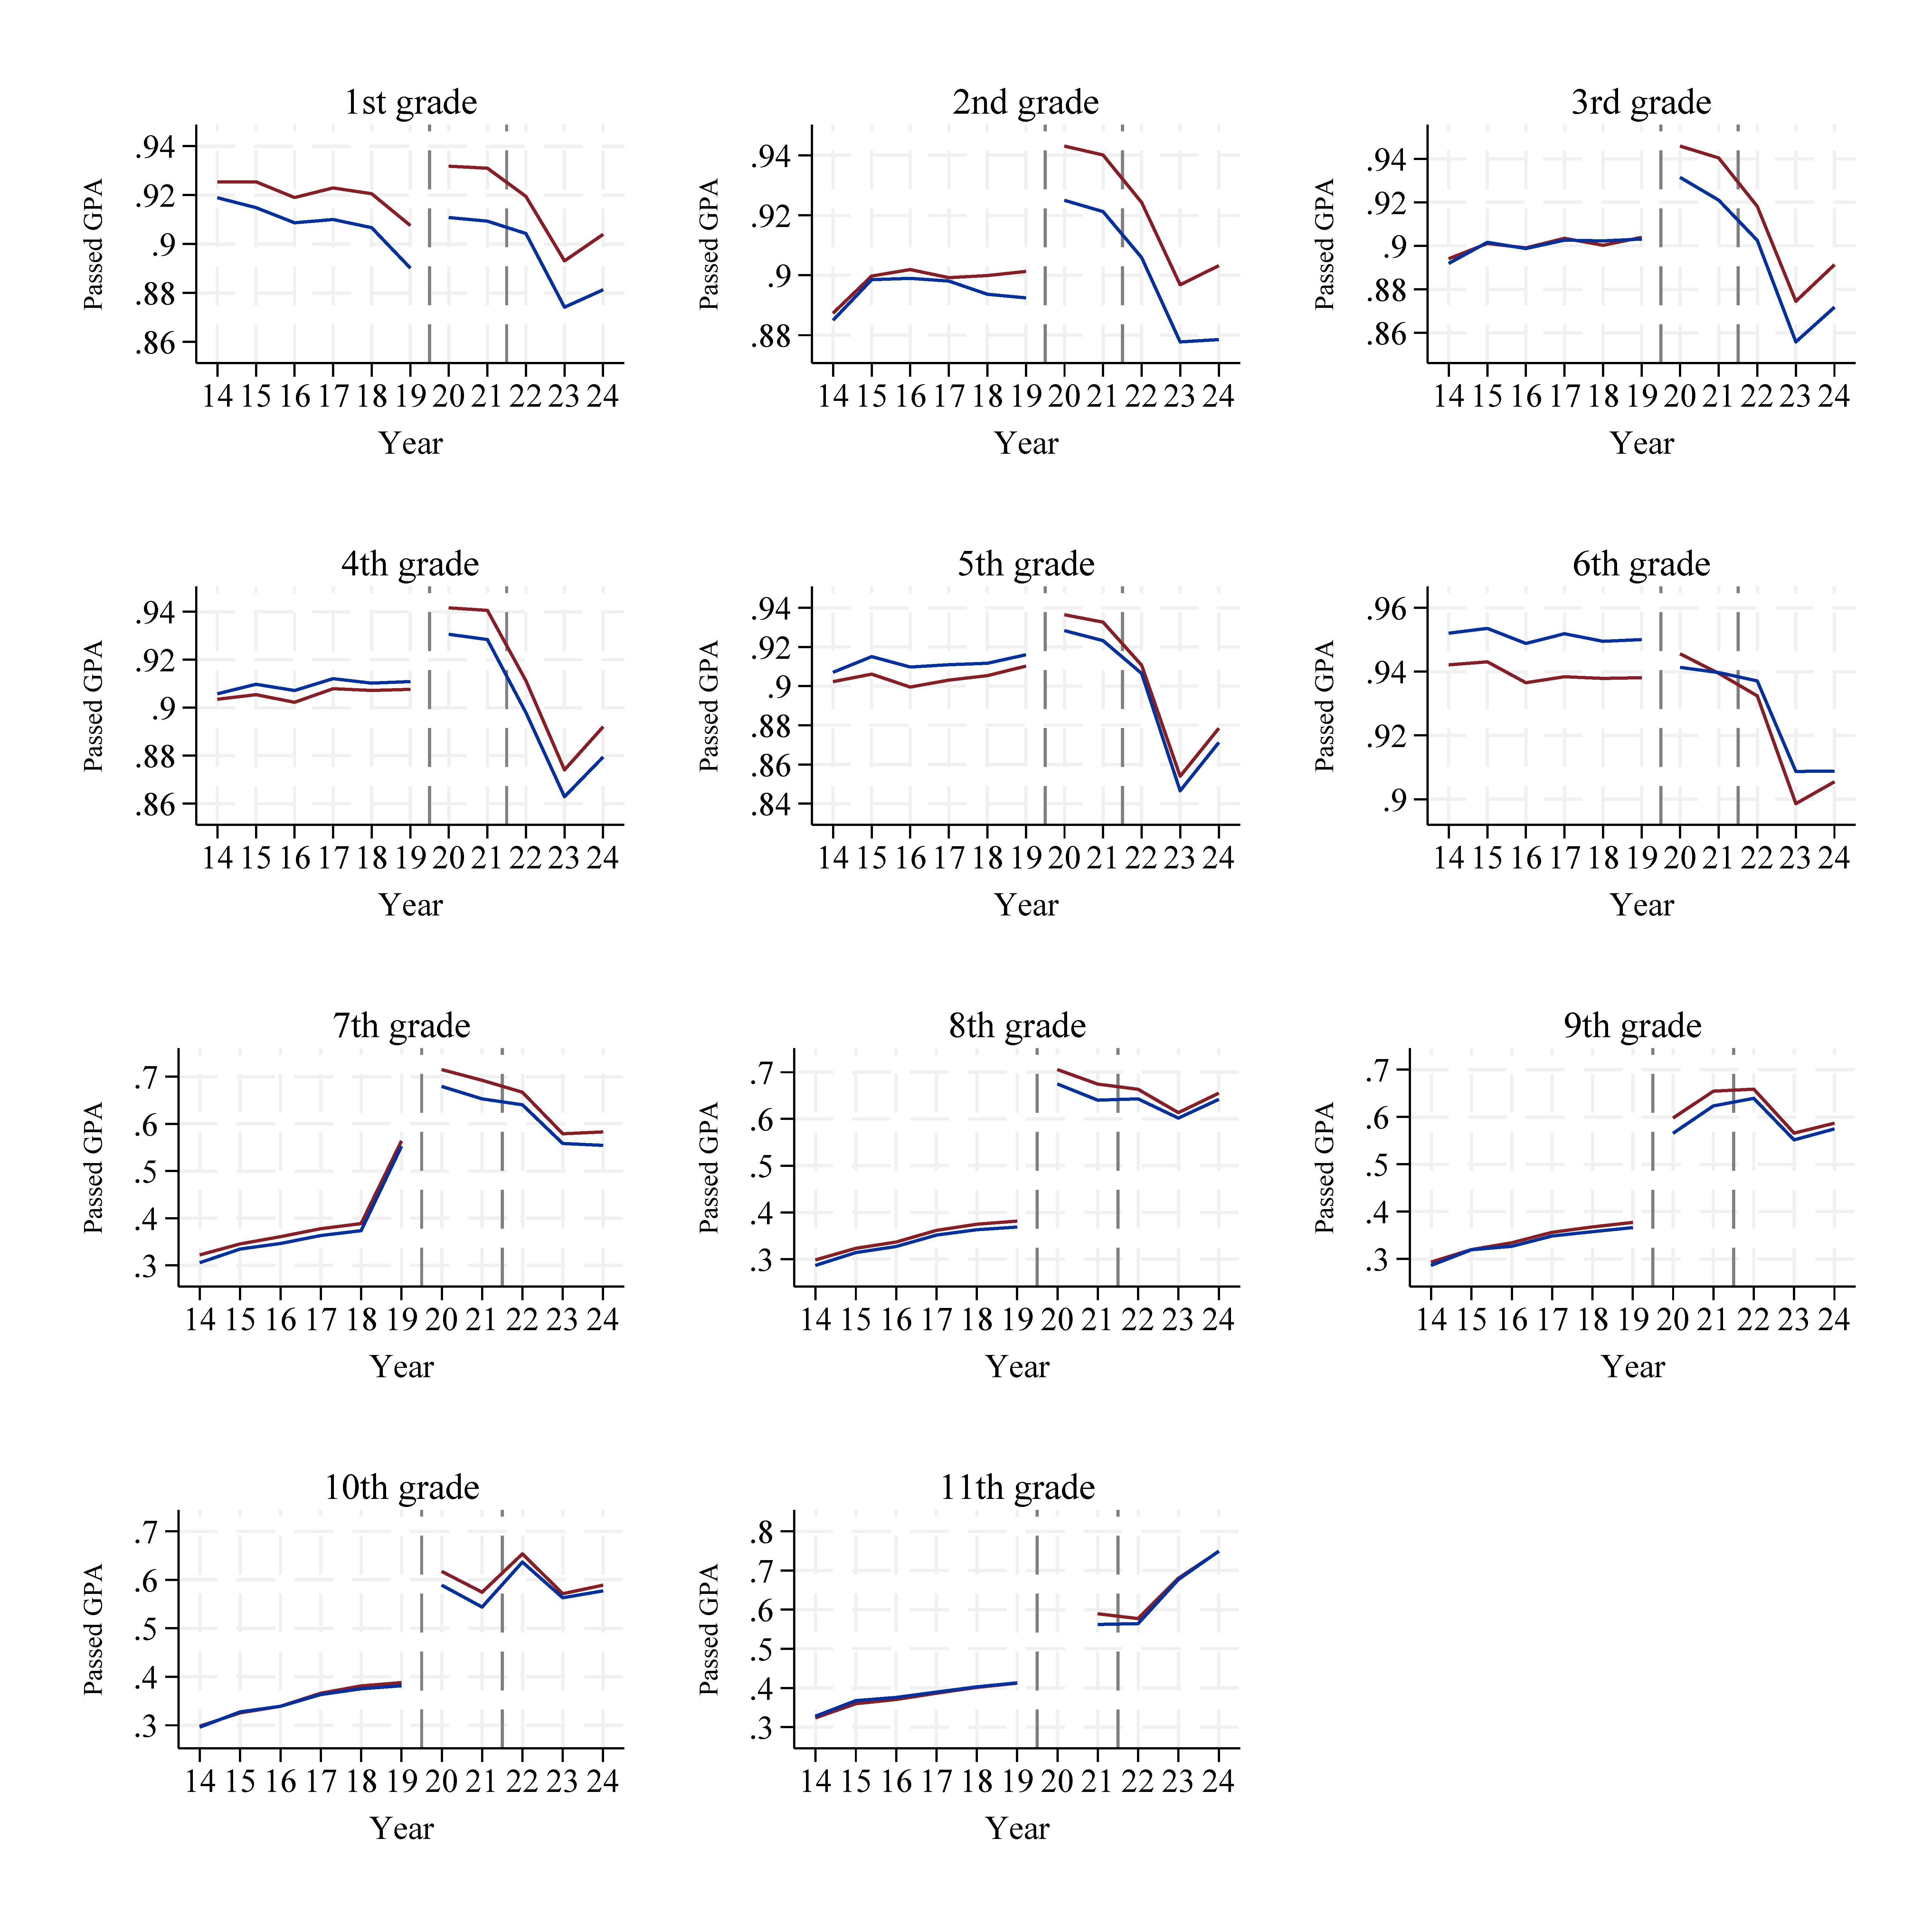
\includegraphics[width=\textwidth]{./FIGURES/Descriptive/raw_grades_pass_math_siblings.pdf}
        \caption{\% of students with an A in Mathematics for each grade 1st-1th}
        \label{fig:trend_pass_grades}
\end{figure}

\begin{figure}[htbp]
         \centering
        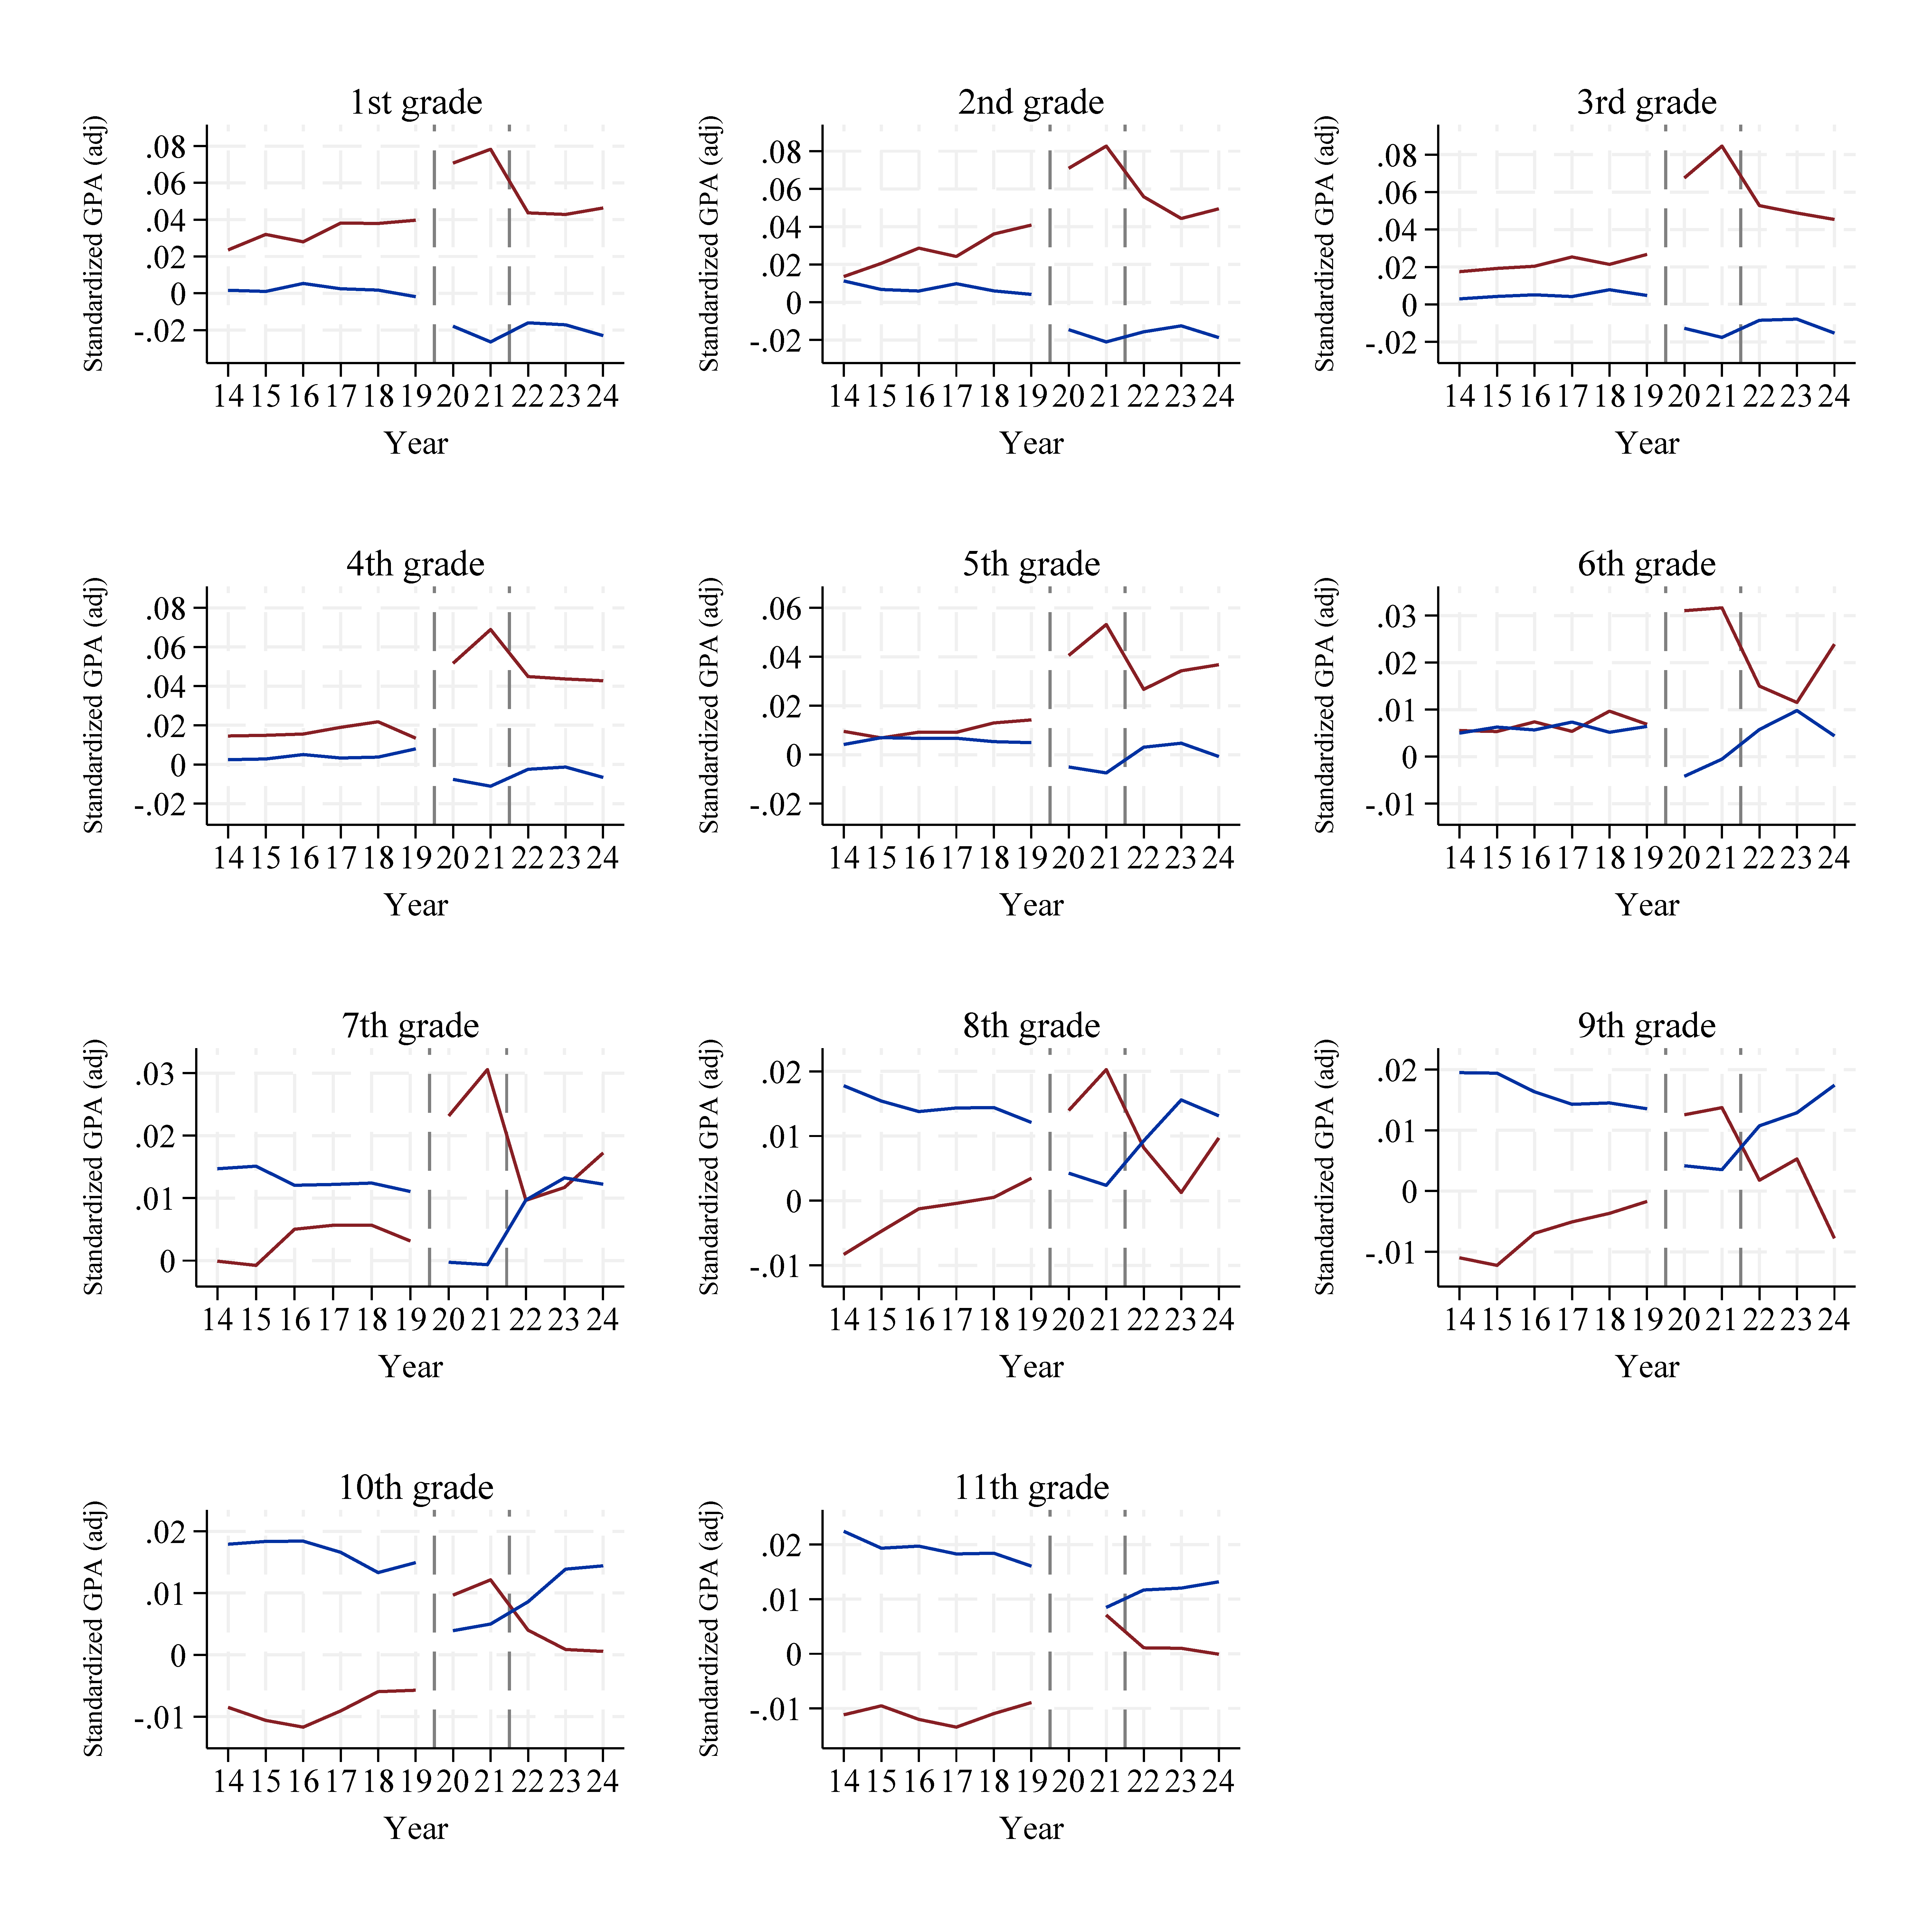
\includegraphics[width=\textwidth]{./FIGURES/Descriptive/raw_grades_std_gpa_m_adj_siblings.pdf}
        \caption{Average GPA standardized within school-grade-year for each grade 1st-1th}
        \label{fig:trend_gpa_grades}
\end{figure}



\begin{figure}[htbp]
    \centering
    
        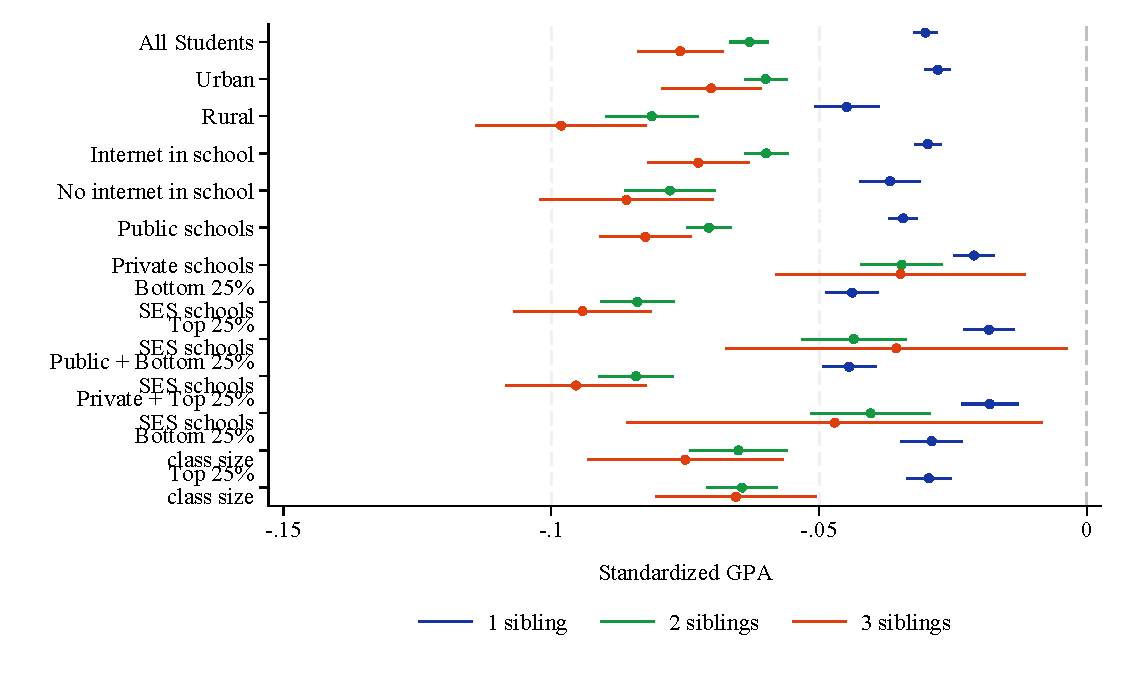
\includegraphics[width=\textwidth]{./FIGURES/TWFE/covid_twfe_A_bysibs_elm_all_gpa_m_adj_Tsiblings_Soldest_4.pdf}
        \caption{Change in gap between children with siblings and only childs}
        \label{fig:fig_appA}

\end{figure}

\begin{figure}[htbp]
    \centering
    
        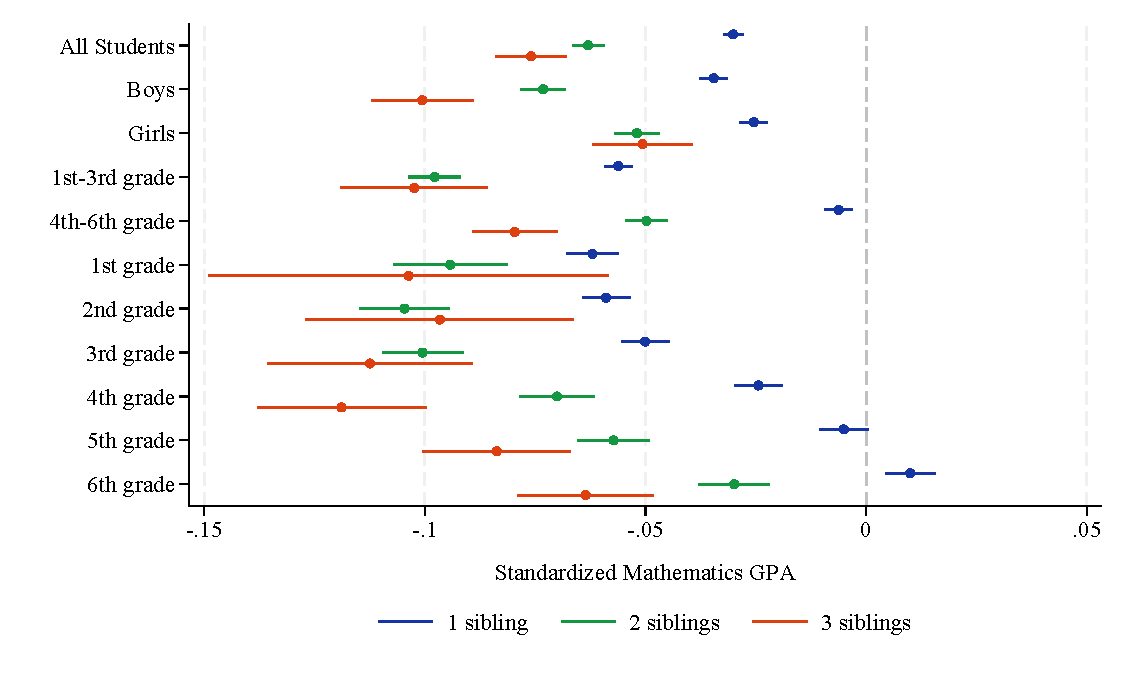
\includegraphics[width=\textwidth]{./FIGURES/TWFE/covid_twfe_B_bysibs_elm_all_gpa_m_adj_Tsiblings_Soldest_4.pdf}
        \caption{Change in gap between children with siblings and only childs}
        \label{fig:fig_appB}

\end{figure}

\begin{figure}[htbp]
    \centering
    
        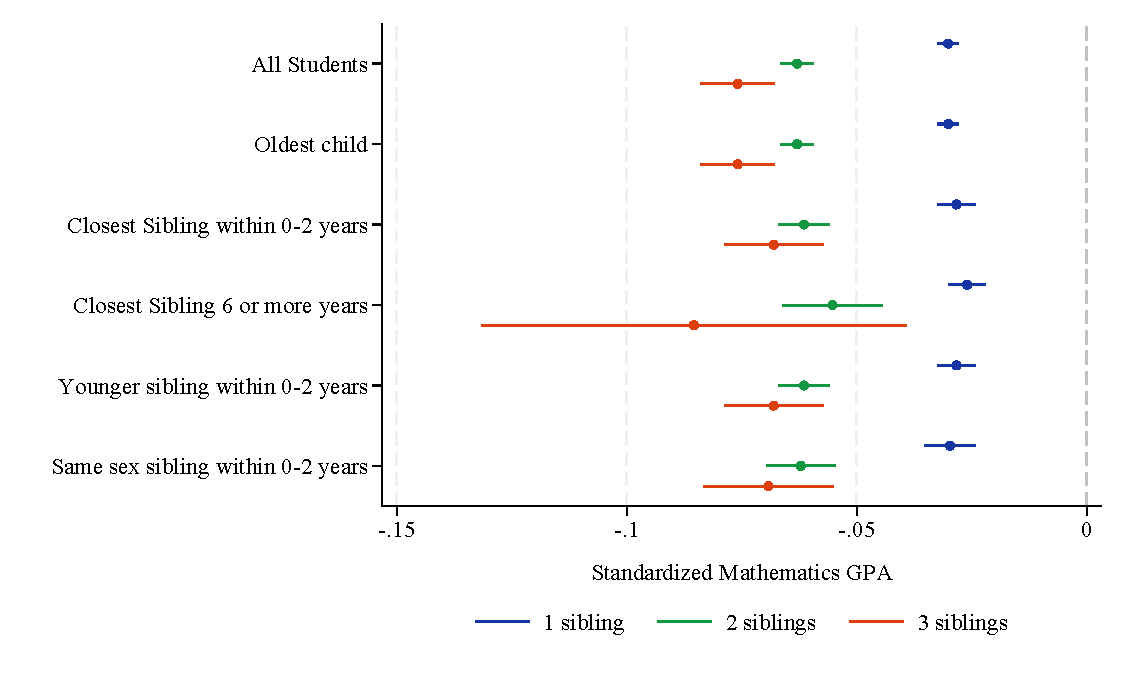
\includegraphics[width=\textwidth]{./FIGURES/TWFE/covid_twfe_C_bysibs_elm_all_gpa_m_adj_Tsiblings_Soldest_4.pdf}
        \caption{Change in gap between children with siblings and only childs}
        \label{fig:fig_appC}

\end{figure}


\begin{figure}[htbp]
    \centering
    
        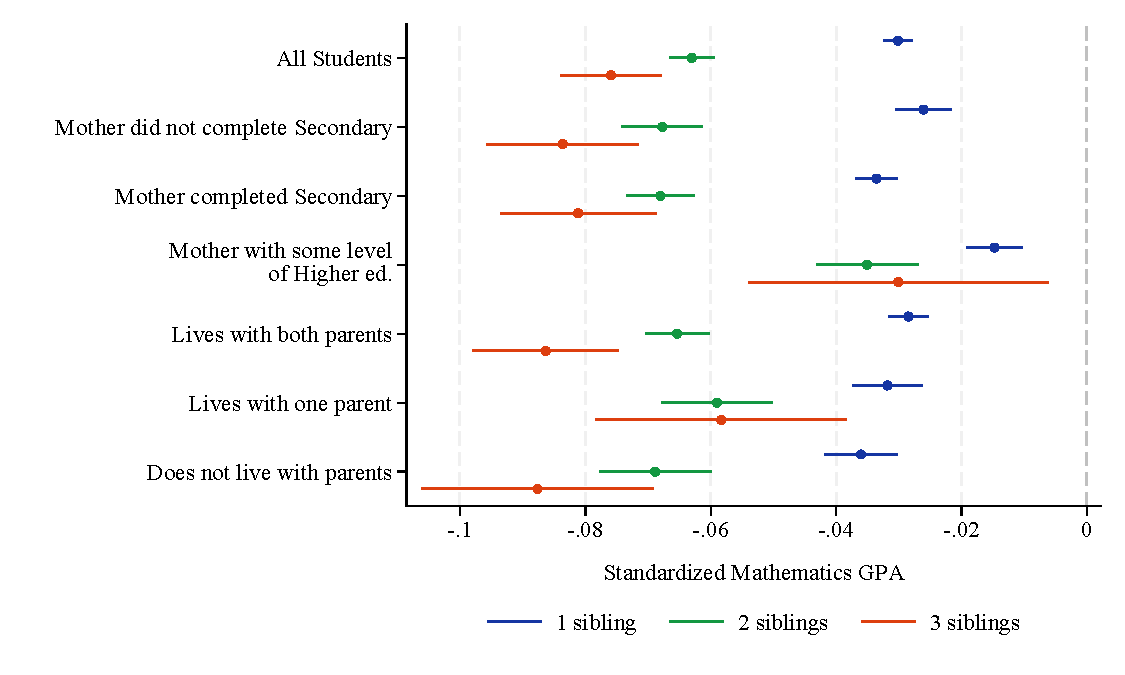
\includegraphics[width=\textwidth]{./FIGURES/TWFE/covid_twfe_D_bysibs_elm_all_gpa_m_adj_Tsiblings_Soldest_4.pdf}
        \caption{Change in gap between children with siblings and only childs}
        \label{fig:fig_appD}

\end{figure}



\end{document}

